\chapter{Implementation} \label{ch:implementation}

\section{Design and Architecture}
The design of the implementation leverages a microservices architecture to simulate real-world data collection and processing. The system was designed to emulate a sensor-driven environment, utilizing containerized services for data generation, communication, transformation, and visualization.

To simulate real sensors or microcontrollers, a Bash application was developed. This application processes a real dataset of air quality data and extracts the data corresponding to specific timestamps. The extracted data is then published to an MQTT broker. This Bash application is packaged in a Docker image to enable scalability and reusability. Multiple instances of this sensor simulation image are deployed as separate Docker containers, each simulating an independent sensor.

To enable communication using the MQTT protocol between the simulated sensors and the data-processing layer, an MQTT broker was deployed. The MQTT broker, also packaged in a Docker container, receives data from the sensor containers and forwards it to the subscribed clients.

A controller service was implemented as a Python application. This application subscribes to the MQTT topics published by the sensors, processes the incoming data, and converts it into a format compatible with Prometheus. The transformed data is then exposed through an HTTP endpoint. The controller application is also containerized and deployed as a separate Docker container.

Prometheus was deployed in a Docker container and configured to periodically scrape the data exposed by the controller service and to retain it for an appropriate amount of time.

Finally, Grafana was deployed as the visualization layer of the system, again in its own Docker container. Grafana was configured to use Prometheus as its data source. Custom dashboards were created to visualize the air quality data collected from the simulated sensors, enabling real-time monitoring and analysis.

The entire system was deployed using Docker Compose to allow for a easy orchestration and management of all the containerized services and for a straightforward, scalable and reproducible deployment.

\begin{figure}[!h]
    \graphicspath{ {./diagrams/} }
    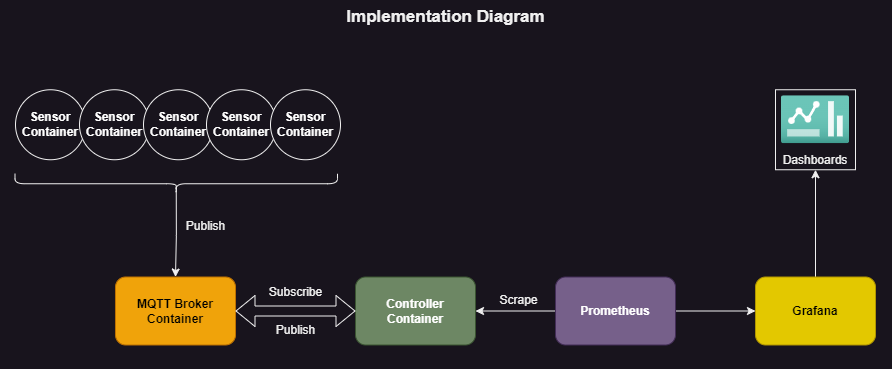
\includegraphics[scale=0.55]{implementation.png}
    \centering
    \caption{Implementation Diagram}
    \label{fig:imple_dia}
\end{figure}

\section{Dataset}
The dataset used contains the responses of a gas multisensor device deployes on the field in an Italian city. Hourly responses averages are recorded along with gas concentrations references from a certified analyzer. The dataset contains 9357 instances of hourly averaged responses from an array of 5 metal oxide chemical sensors embedded in an Air Quality Chemical Multisensor Device. Ground Truth hourly averaged concentrations for CO, Non Metanic Hydrocarbons, Benzene, Total Nitrogen Oxides (NOx) and Nitrogen Dioxide (NO2) were provided by a co-located reference certified analyzer.

\begin{table}[!h]
\begin{tabular}{|c|p{0.8\linewidth}|}
    \hline
    \multicolumn{2}{|c|}{\textbf{Attribute Information}} \\
    \hline
    \hline
    0& Date (DD/MM/YYYY) \\ \hline
    1& Time (HH.MM.SS) \\ \hline
    2& True hourly averaged concentration CO in $mg/m^3$ (reference analyzer) \\ \hline
    3& PT08.S1 (tin oxide) hourly averaged sensor response (nominally CO targeted) \\ \hline
    4& True hourly averaged overall Non Metanic HydroCarbons concentration in $microg/m^3$ (reference analyzer) \\ \hline
    5& True hourly averaged Benzene concentration in $microg/m^3$ (reference analyzer) \\ \hline
    6& PT08.S2 (titania) hourly averaged sensor response (nominally NMHC targeted) \\ \hline
    7& True hourly averaged NOx concentration in ppb (reference analyzer) \\ \hline
    8& PT08.S3 (tungsten oxide) hourly averaged sensor response (nominally NOx targeted) \\ \hline
    9& True hourly averaged NO2 concentration in $microg/m^3$ (reference analyzer) \\ \hline
    10& PT08.S4 (tungsten oxide) hourly averaged sensor response (nominally NO2 targeted) \\ \hline
    11& PT08.S5 (indium oxide) hourly averaged sensor response (nominally O3 targeted) \\ \hline
    12& Temperature in °C \\ \hline
    13& Relative Humidity (\%) \\ \hline
    14& AH Absolute Humidity  \\ \hline
\end{tabular}
\centering
\caption{Dataset Attribute Information}
\label{fig:dataset_attri}
\end{table}

\section{Sensor Simulator}

\section{MQTT Broker}

\section{Controller Node}

\section{Prometheus}

\section{Grafana}

\section{Orchestration}
